\documentclass[xetex,mathserif,serif]{beamer}
\usepackage{polyglossia}
\setdefaultlanguage[babelshorthands=true]{russian}
\usepackage{minted}
\usepackage{tabu}
\usepackage{forest}

\usepackage{textpos}
\setlength{\TPHorizModule}{1cm}
\setlength{\TPVertModule}{1cm}

\usetikzlibrary{arrows}

\useoutertheme{infolines}

\setmainfont{FreeSans}
\newfontfamily{\russianfonttt}{FreeSans}

\definecolor{links}{HTML}{2A1B81}
\hypersetup{colorlinks,linkcolor=,urlcolor=links}

\tabulinesep=1.2mm

\newcommand{\attribution}[1] {
	\begin{flushright}\begin{scriptsize}\textcolor{gray}{\textcopyright\, #1}\end{scriptsize}\end{flushright}
}

\title{Событийно-ориентированное программирование}
\author[Юрий Литвинов]{Юрий Литвинов \newline \textcolor{gray}{\small\texttt{yurii.litvinov@gmail.com}}}
\date{02.03.2018г}

\begin{document}
	
	\frame{\titlepage}

	\begin{frame}
		\frametitle{Событийно-ориентированное программирование: зачем?}
		\begin{itemize}
			\item Большая часть приложений большую часть времени чего-то ждёт
			\item Активное ожидание потребляет системные ресурсы
			\item Приложения с пользовательским интерфейсом:
			\begin{itemize}
				\item Цикл обработки событий
				\item Очередь событий
				\item Обработчики
			\end{itemize}
			\item Сетевые и распределённые приложения
			\item Приложения, работающие с оборудованием
		\end{itemize}
	\end{frame}

	\begin{frame}
		\frametitle{Реализация}
		\begin{itemize}
			\item Callback-и (hooks)
			\item Переопределение виртуальных методов библиотечного класса
			\begin{itemize}
				\item Inversion of Control --- не мы вызываем библиотеку, а она нас
			\end{itemize}
			\item Языковая поддержка --- event-ы
			\item Паттерн ``Наблюдатель''
		\end{itemize}
	\end{frame}

	\begin{frame}
		\frametitle{Паттерн ``Наблюдатель''}
		\begin{center}
			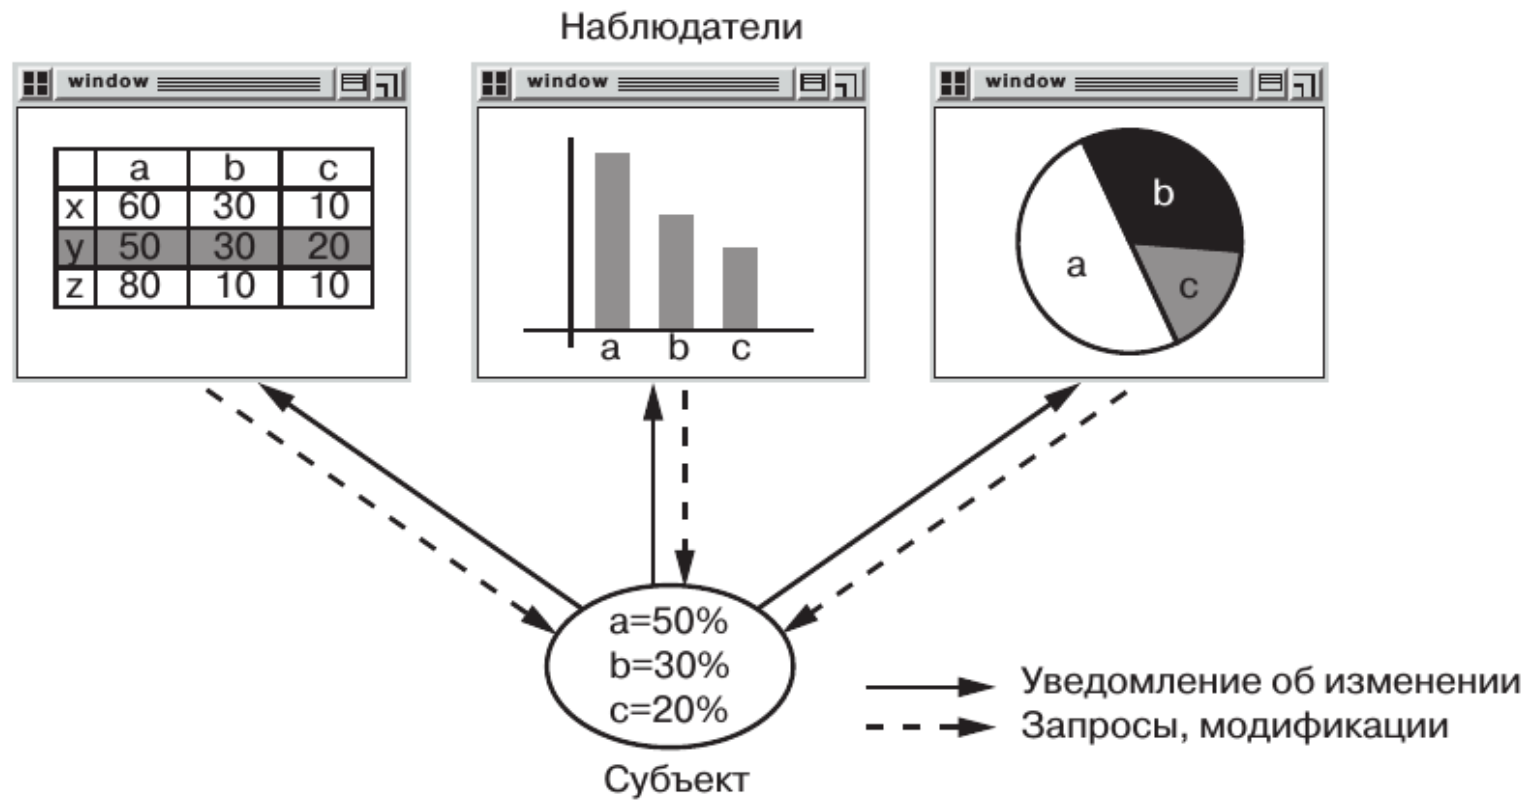
\includegraphics[width=0.9\textwidth]{observerExample.png}
		\end{center}
	\end{frame}

	\begin{frame}
		\frametitle{Наблюдатель, структура классов}
		\begin{center}
			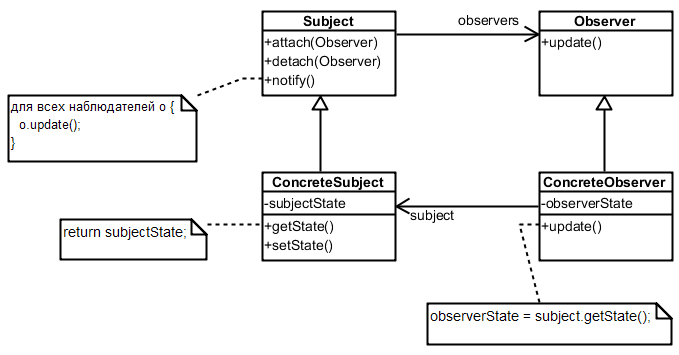
\includegraphics[width=0.8\textwidth]{observer.png}
		\end{center}
	\end{frame}

	\begin{frame}[fragile]
		\frametitle{Пример, кнопки в JavaFX}
		\begin{small}
			\begin{minted}{java}
public class Buttons extends Application  {
    @Override
    public void start(Stage primaryStage) throws Exception {
        Button button = new Button("Click me");

        button.setOnAction(new EventHandler<ActionEvent>() {
            @Override
            public void handle(ActionEvent event) {
                Platform.exit();
            }
        });

        Scene scene = new Scene(button, 200, 100);
        primaryStage.setScene(scene);
        primaryStage.show();
    }
}
			\end{minted}
		\end{small}
	\end{frame}

	\begin{frame}[fragile]
		\frametitle{Языковая поддержка: event-ы в C\#}
		\begin{itemize}
			\item Ключевое слово \textbf{event}, декларирующее событие:

				\begin{minted}{csharp}
public event Action SomethingHappened;
				\end{minted}
			\item На событие можно подписаться:

				\begin{minted}{csharp}
ourObject.SomethingHappened += DoSomething;
				\end{minted}
			\item И отписаться:

				\begin{minted}{csharp}
ourObject.SomethingHappened -= DoSomething;
				\end{minted}
			\item А ещё событие можно инициировать:

				\begin{minted}{csharp}
SomethingHappened?.Invoke();
				\end{minted}
		\end{itemize}
	\end{frame}

	\begin{frame}[fragile]
		\frametitle{Пример, консольная игра}
		\framesubtitle{EventLoop}
		\begin{scriptsize}
			\begin{minted}{csharp}
public class EventLoop
{
    public event Action OnLeft;
    public event Action OnRight;

    public void Run()
    {
        while (true)
        {
            var key = Console.ReadKey(true);
            switch (key.Key)
            {
                case ConsoleKey.LeftArrow:
                    OnLeft?.Invoke();
                    break;
                case ConsoleKey.RightArrow:
                    OnRight?.Invoke();
                    break;
            }
        }
    }
}
			\end{minted}
		\end{scriptsize}
	\end{frame}

	\begin{frame}[fragile]
		\frametitle{Пример, консольная игра}
		\framesubtitle{Game}
		\begin{minted}{csharp}
public class Game
{
    public void OnLeft()
        => Console.CursorLeft--;

    public void OnRight()
        => Console.CursorLeft++;
}
		\end{minted}
	\end{frame}

	\begin{frame}[fragile]
		\frametitle{Пример, консольная игра}
		\framesubtitle{Main}
		\begin{minted}{csharp}
public class Program
{
    public static void Main(string[] args)
    {
        var eventLoop = new EventLoop();
        var game = new Game();

        eventLoop.OnLeft += game.OnLeft;
        eventLoop.OnRight += game.OnRight;
        eventLoop.Run();
    }
}
		\end{minted}
	\end{frame}

	\begin{frame}
		\frametitle{C++/Qt --- сигналы и слоты}
		\begin{center}
			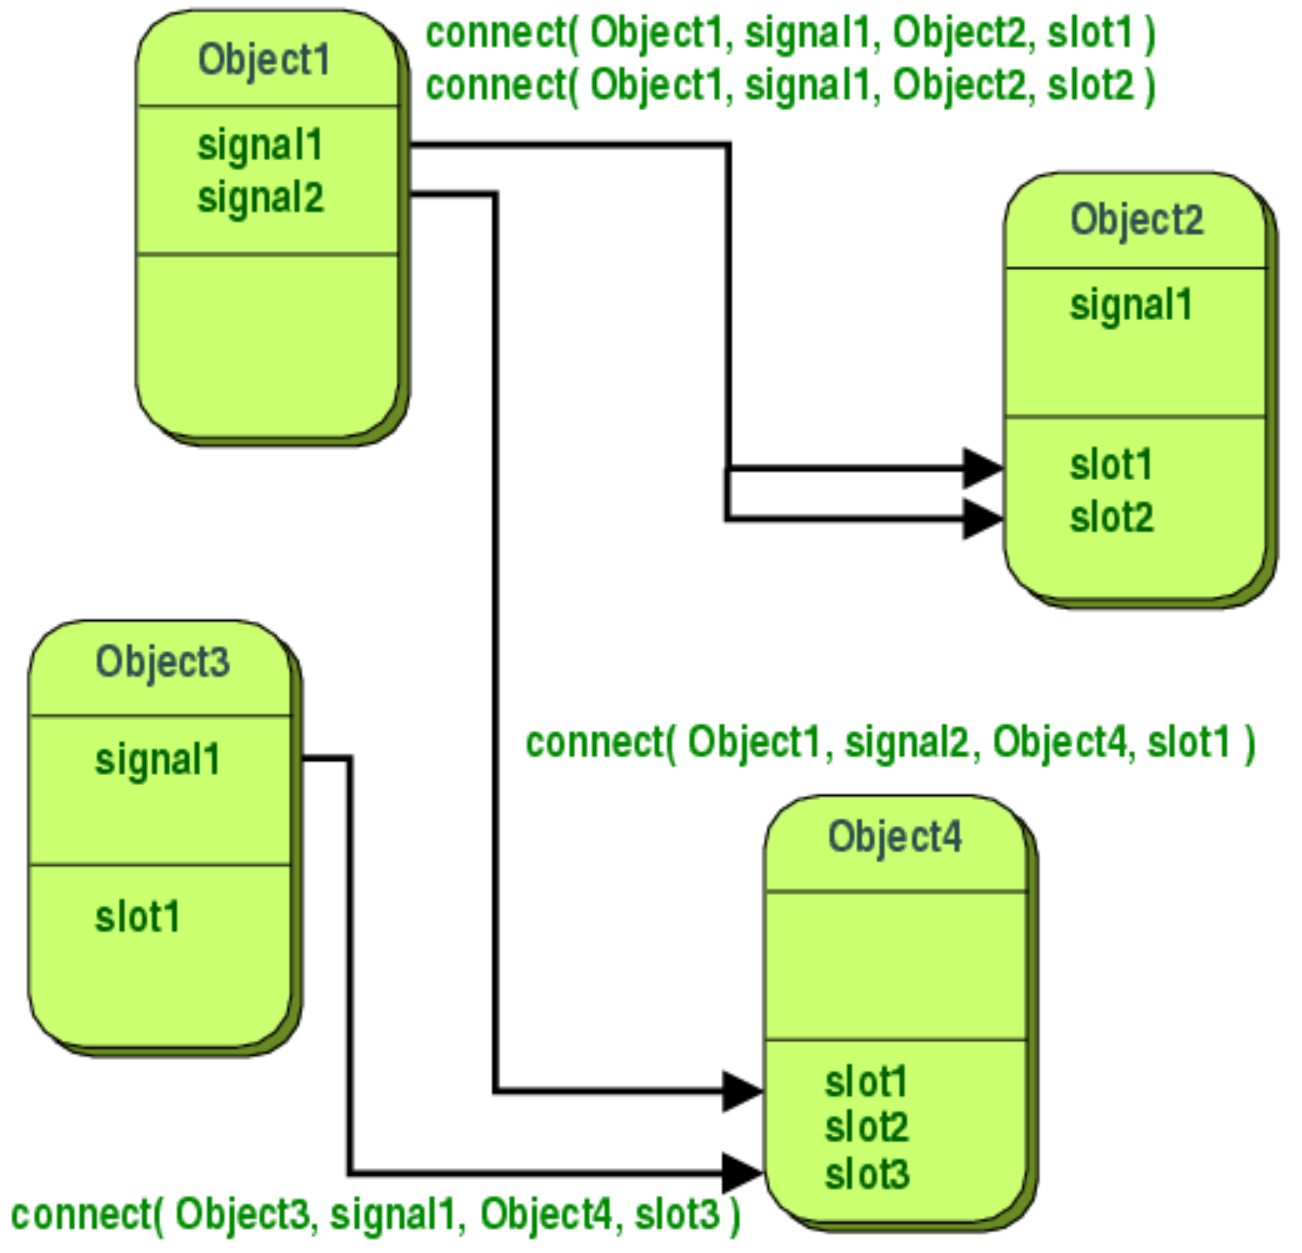
\includegraphics[width=0.6\textwidth]{signalsSlots.png}
		\end{center}
	\end{frame}

	\begin{frame}[fragile]
		\frametitle{Пример}
		\begin{scriptsize}
			\begin{minted}{c++}
#include <QObject>

class Counter : public QObject
{
    Q_OBJECT

public:
    Counter() { m_value = 0; }

    int value() const { return m_value; }

public slots:
    void setValue(int value);

signals:
    void valueChanged(int newValue);

private:
    int m_value;
};
			\end{minted}
		\end{scriptsize}
	\end{frame}

	\begin{frame}
		\frametitle{Пример событийной архитектуры --- ROS}
		\begin{center}
			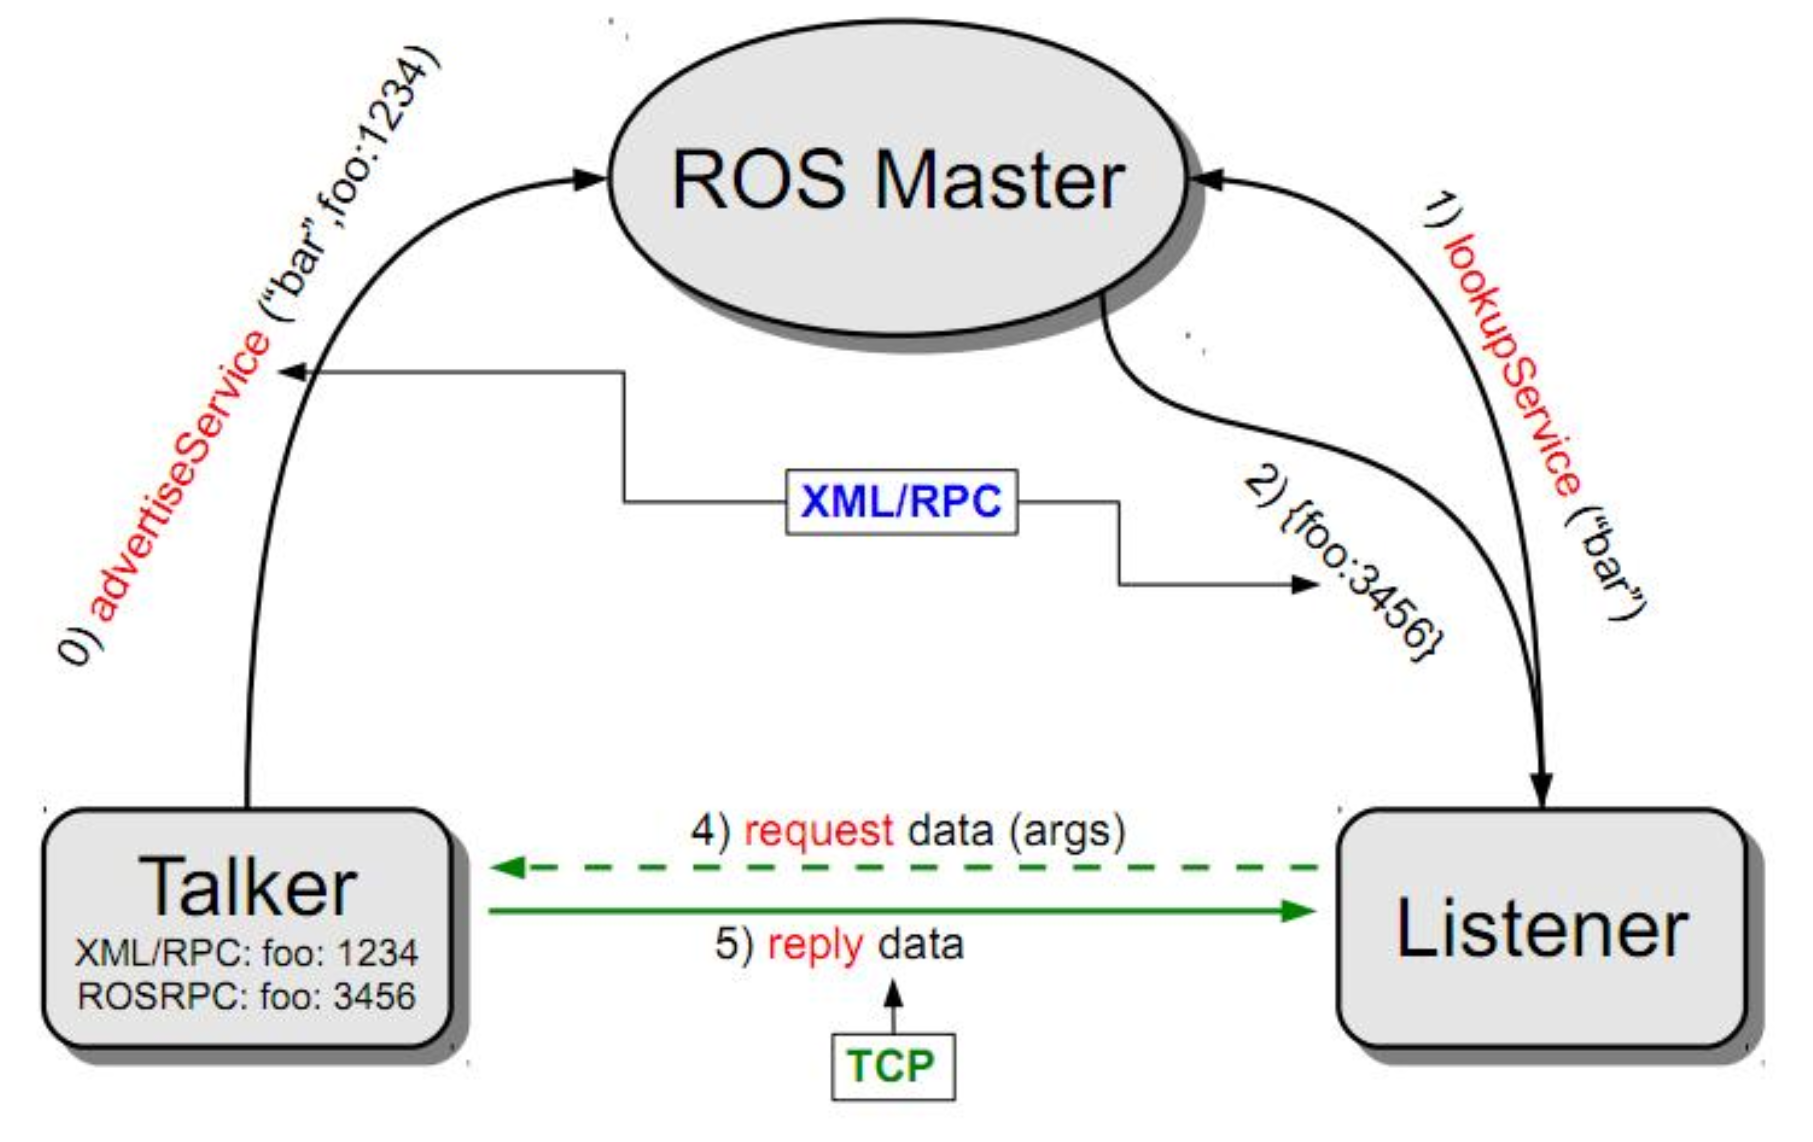
\includegraphics[width=0.8\textwidth]{ros.png}
		\end{center}
	\end{frame}

\end{document}